\subsection{Valg af standard komponenter} \label{Standard komponenter}
Stellet laves af standard komponenter, for at opfylde præstations krav 11 og 12 om antal værktøj der skal benyttes til at samle robotten, samt minimere omkostninger til produktion af enkelt komponenter. Der gøres brug af $\SI{40}{mm}\times\SI{40}{mm}$ aluminiums t-slots profiler, som ses i figur \ref{fig:T-slot profil 1}. T-slot profiler (også kendt som aluminiumsprofilrammer) er kendetegnet ved de åbne T-formede spor langs deres sider, som tillader ned og fleksible montering af beslag, skruer og andre komponenter. Dette gør dem særligt velegnet til maskinstel, arbejdsstationer og robotsystemer, hvor modularitet og præcision ønskes. Aluminium T-slot profilrør leveres i standard størreler, hvortil diverse standard T-slots beslag og notsten kan tilkøbes. \parencite{McMaster-Carr2025T-slottedFraming}

\begin{figure}[H]
    \centering
    \begin{subfigure}[b]{0.34\textwidth}
        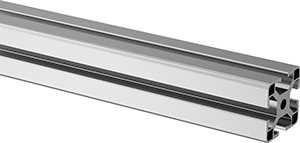
\includegraphics[width=\textwidth]{Sections/6 Detaljeløsning/Media/T-slots.png}
        \caption{Alu T-slot profilrør.} 
        \label{fig:T-slot profil 1}
    \end{subfigure}
    \hfill
    \begin{subfigure}[b]{0.4\textwidth}
       \centering
        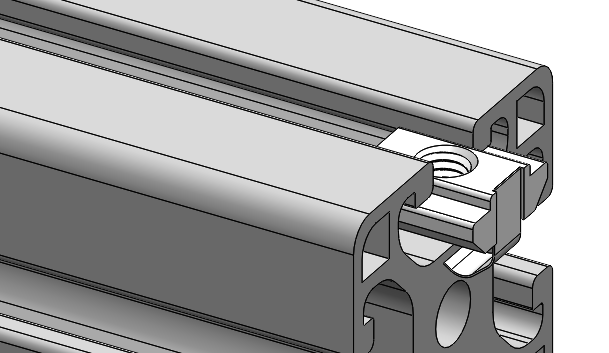
\includegraphics[width=.9\textwidth]{Sections/6 Detaljeløsning/Media/T-slot med Notsten.png}
        \caption{Alu T-slot profilrør med notsten} 
        \label{fig: T-slot profil med notsten}
    \end{subfigure}
     \hfill
    \begin{subfigure}[b]{0.24\textwidth}
        \centering
        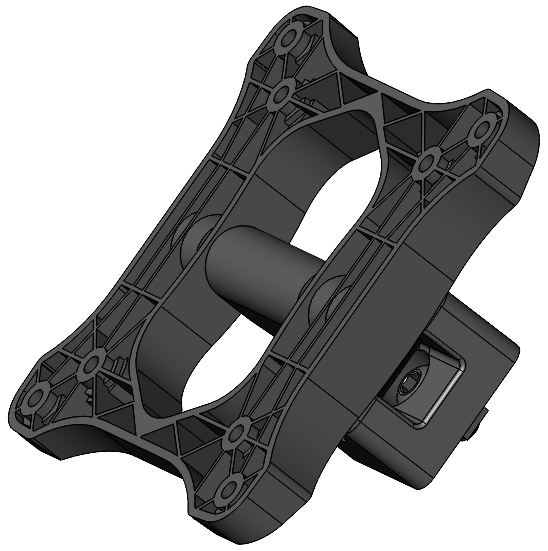
\includegraphics[width=.9\textwidth]{Sections/6 Detaljeløsning/Media/kontrolsystem montage1.png}
         \caption{Monterings element}
    \label{fig:T-slot tablet holder}
    \end{subfigure}
    \caption{T-slot profil rør med notsten og monterings element. \textit{(c)} er til montering af elektronik efter VESA (Video Electronics Standards Association) til standard i T-slot alu profilrør. Billeder fra \parencite{McMaster-Carr2025T-SlottedRails}}
\end{figure} \plainbreak{-1}

Aluminium T-slot profilrør gør det muligt, at montere kontrolsystemet alle steder på stellet, hvor der ikke er beslag. Montage sker ved at indsætte notsten i t-slotten, som set på figur \ref{fig: T-slot profil med notsten}, hvor bolte kan skrues i. Kamera og skærm kan for eksempel monteres ved brug af monterings elementer, som det der kan ses i figur \ref{fig:T-slot tablet holder}. \parencite{McMaster-Carr2025T-slottedFraming}.





%I konstruktionen af stellet er der brugt t-slot aluminiumsrammer. Til påsætning er det derfor muligt, at montere midler med t-slot ender på stellet. Denne monteringsmetode gør det muligt at sætte mange forskellige monteringsmidler til forskellige kameraer og skærme, til kontrolsystemets opgaver.
\begin{comment}
    \begin{figure}[H]
    \centering
    \begin{subfigure}[b]{0.48\textwidth}
        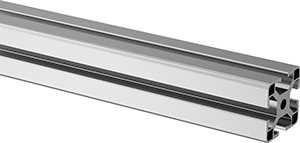
\includegraphics[width=\textwidth]{Sections/6 Detaljeløsning/Media/T-slots.png}
        \caption{Alu T-slot profilrør. \parencite{McMaster-Carr2025T-SlottedRails}} 
       
    \end{subfigure}
    \hfill
    \begin{subfigure}[b]{0.48\textwidth}
    \centering
        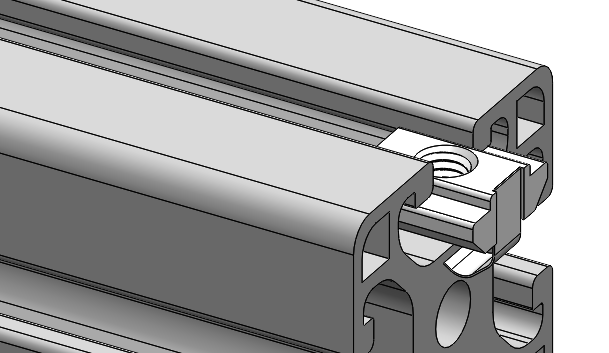
\includegraphics[width=.9\textwidth]{Sections/6 Detaljeløsning/Media/T-slot med Notsten.png}
        \caption{Alu T-slot profilrør med notsten} 
        
    \end{subfigure}
    \caption{}
\end{figure} \plainbreak{-1}


\begin{figure}[H]
    \centering
    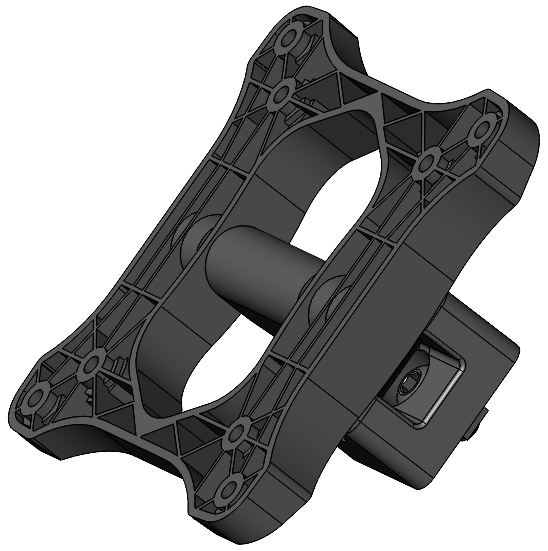
\includegraphics[width=0.3
    \linewidth]{Sections/6 Detaljeløsning/Media/kontrolsystem montage1.png}
    \caption{Montering af elektronik efter VESA (Video Electronics Standards Association) standard i T-slot alu profilrør }
    
\end{figure} \plainbreak{-1}
\end{comment}